\documentclass[12pt,a4paper]{article}

% -------------------------------------------------
% Basic packages
% -------------------------------------------------
\usepackage[a4paper,margin=1in]{geometry}
\usepackage{fontspec}
\usepackage{ctex}
\usepackage{amsmath,amssymb}
\usepackage{graphicx}
\usepackage{booktabs}
\usepackage{array}
\usepackage{longtable}
\usepackage{caption}
\usepackage{float}
\usepackage{setspace}
\usepackage{fancyhdr}
\usepackage{hyperref}
\usepackage{xcolor}
\usepackage{enumitem}
\usepackage{listings}

% -------------------------------------------------
% Table of contents setup
% -------------------------------------------------
\setcounter{tocdepth}{2}

% -------------------------------------------------
% Font setup
% -------------------------------------------------
\setmainfont{Noto Serif}
\setmonofont{DejaVu Sans Mono}

% -------------------------------------------------
% Line spacing and paragraph formatting
% -------------------------------------------------
\onehalfspacing
\setlength{\parindent}{2em}
\setlength{\parskip}{0.4em}

% -------------------------------------------------
% Header / footer
% -------------------------------------------------
\pagestyle{fancy}
\fancyhf{}
\fancyfoot[C]{\thepage}
\renewcommand{\headrulewidth}{0pt}

% -------------------------------------------------
% Hyperref setup
% -------------------------------------------------
\hypersetup{
    colorlinks=true,
    linkcolor=blue,
    urlcolor=blue,
    citecolor=blue
}

% -------------------------------------------------
% Code listing setup
% -------------------------------------------------
\lstset{
    basicstyle=\ttfamily\small,
    breaklines=true,
    frame=single,
    columns=fullflexible,
    showstringspaces=false
}

% -------------------------------------------------
% User-defined information
% -------------------------------------------------
\newcommand{\HomeworkTitle}{Computational Physics Ex\_3}
\newcommand{\StudentID}{2024141230044}
\newcommand{\StudentName}{范奕}

\begin{document}

% =================================================
% Title block
% =================================================
\begin{center}
    {\LARGE \textbf{\HomeworkTitle}}\\[1.2em]
    {\large Student ID: \StudentID}\\[0.5em]
    {\large Name: \StudentName}
\end{center}

\vspace{0.5em}
\noindent\rule{\textwidth}{0.8pt}
\vspace{0.5em}

\section*{Problem 1}

\begin{figure}[H]
    \centering
    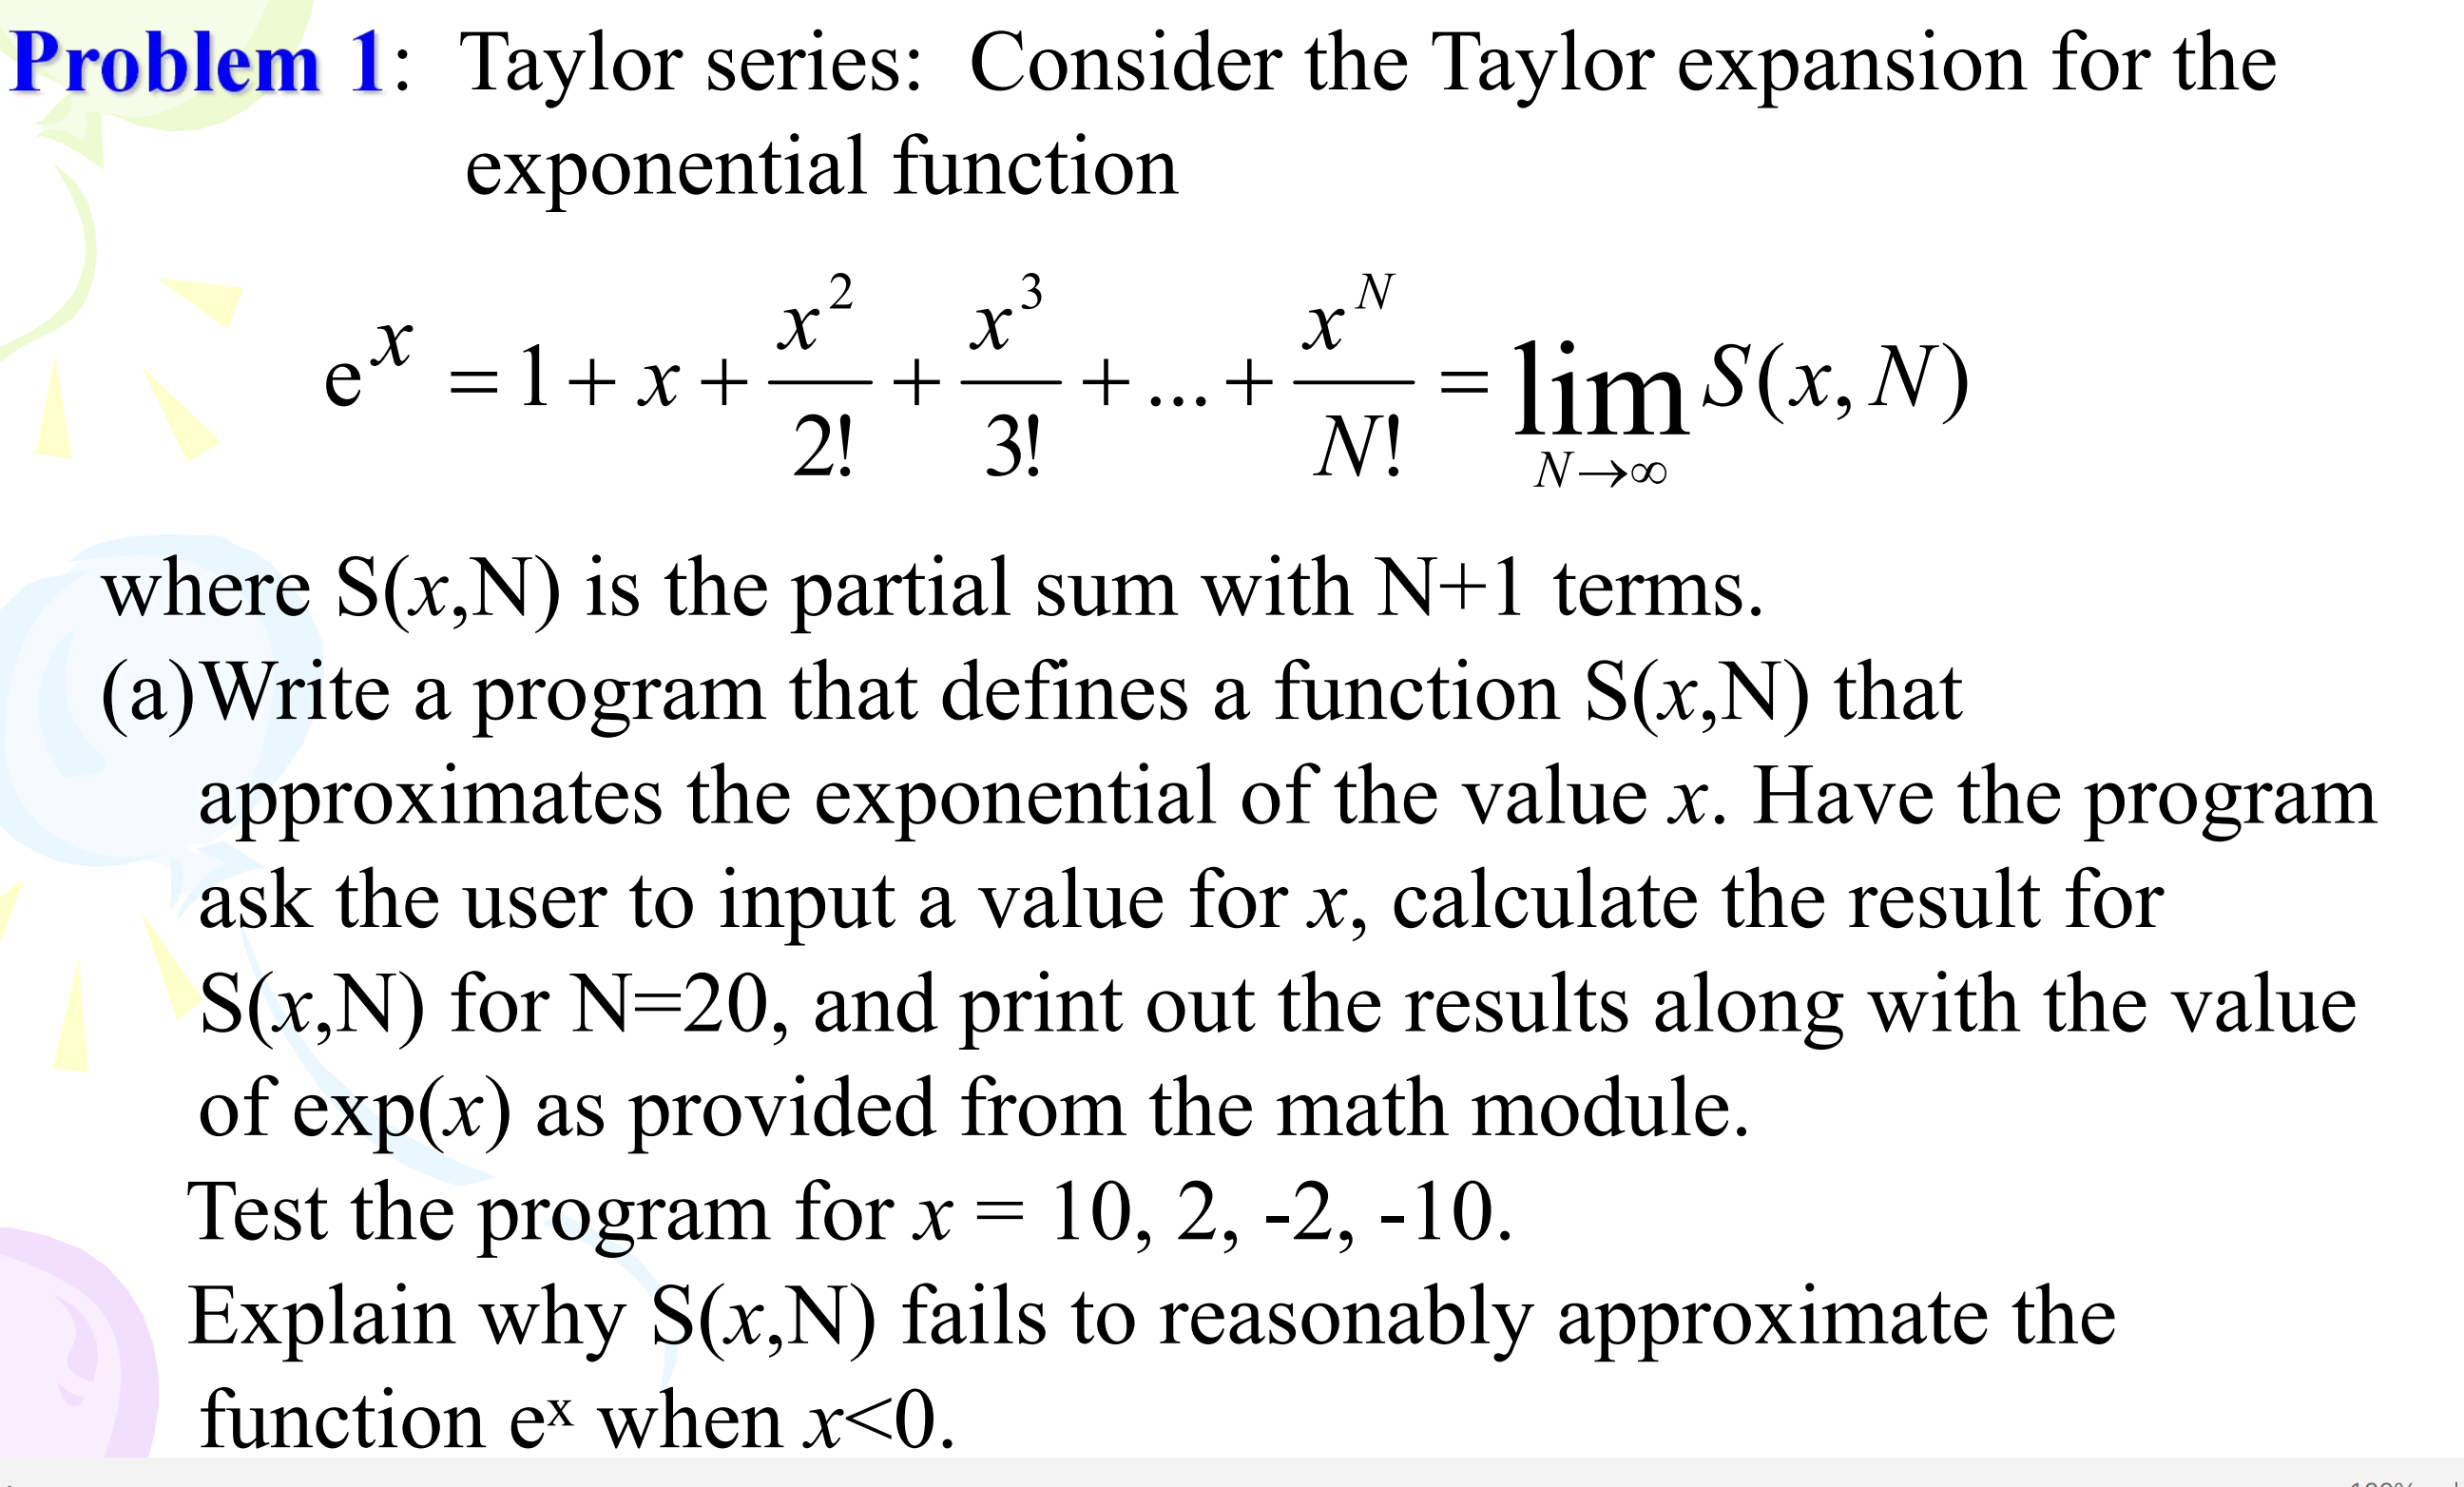
\includegraphics[width=0.8\textwidth]{pic/problem1.png}
\end{figure}

\begin{figure}[H]
    \centering
    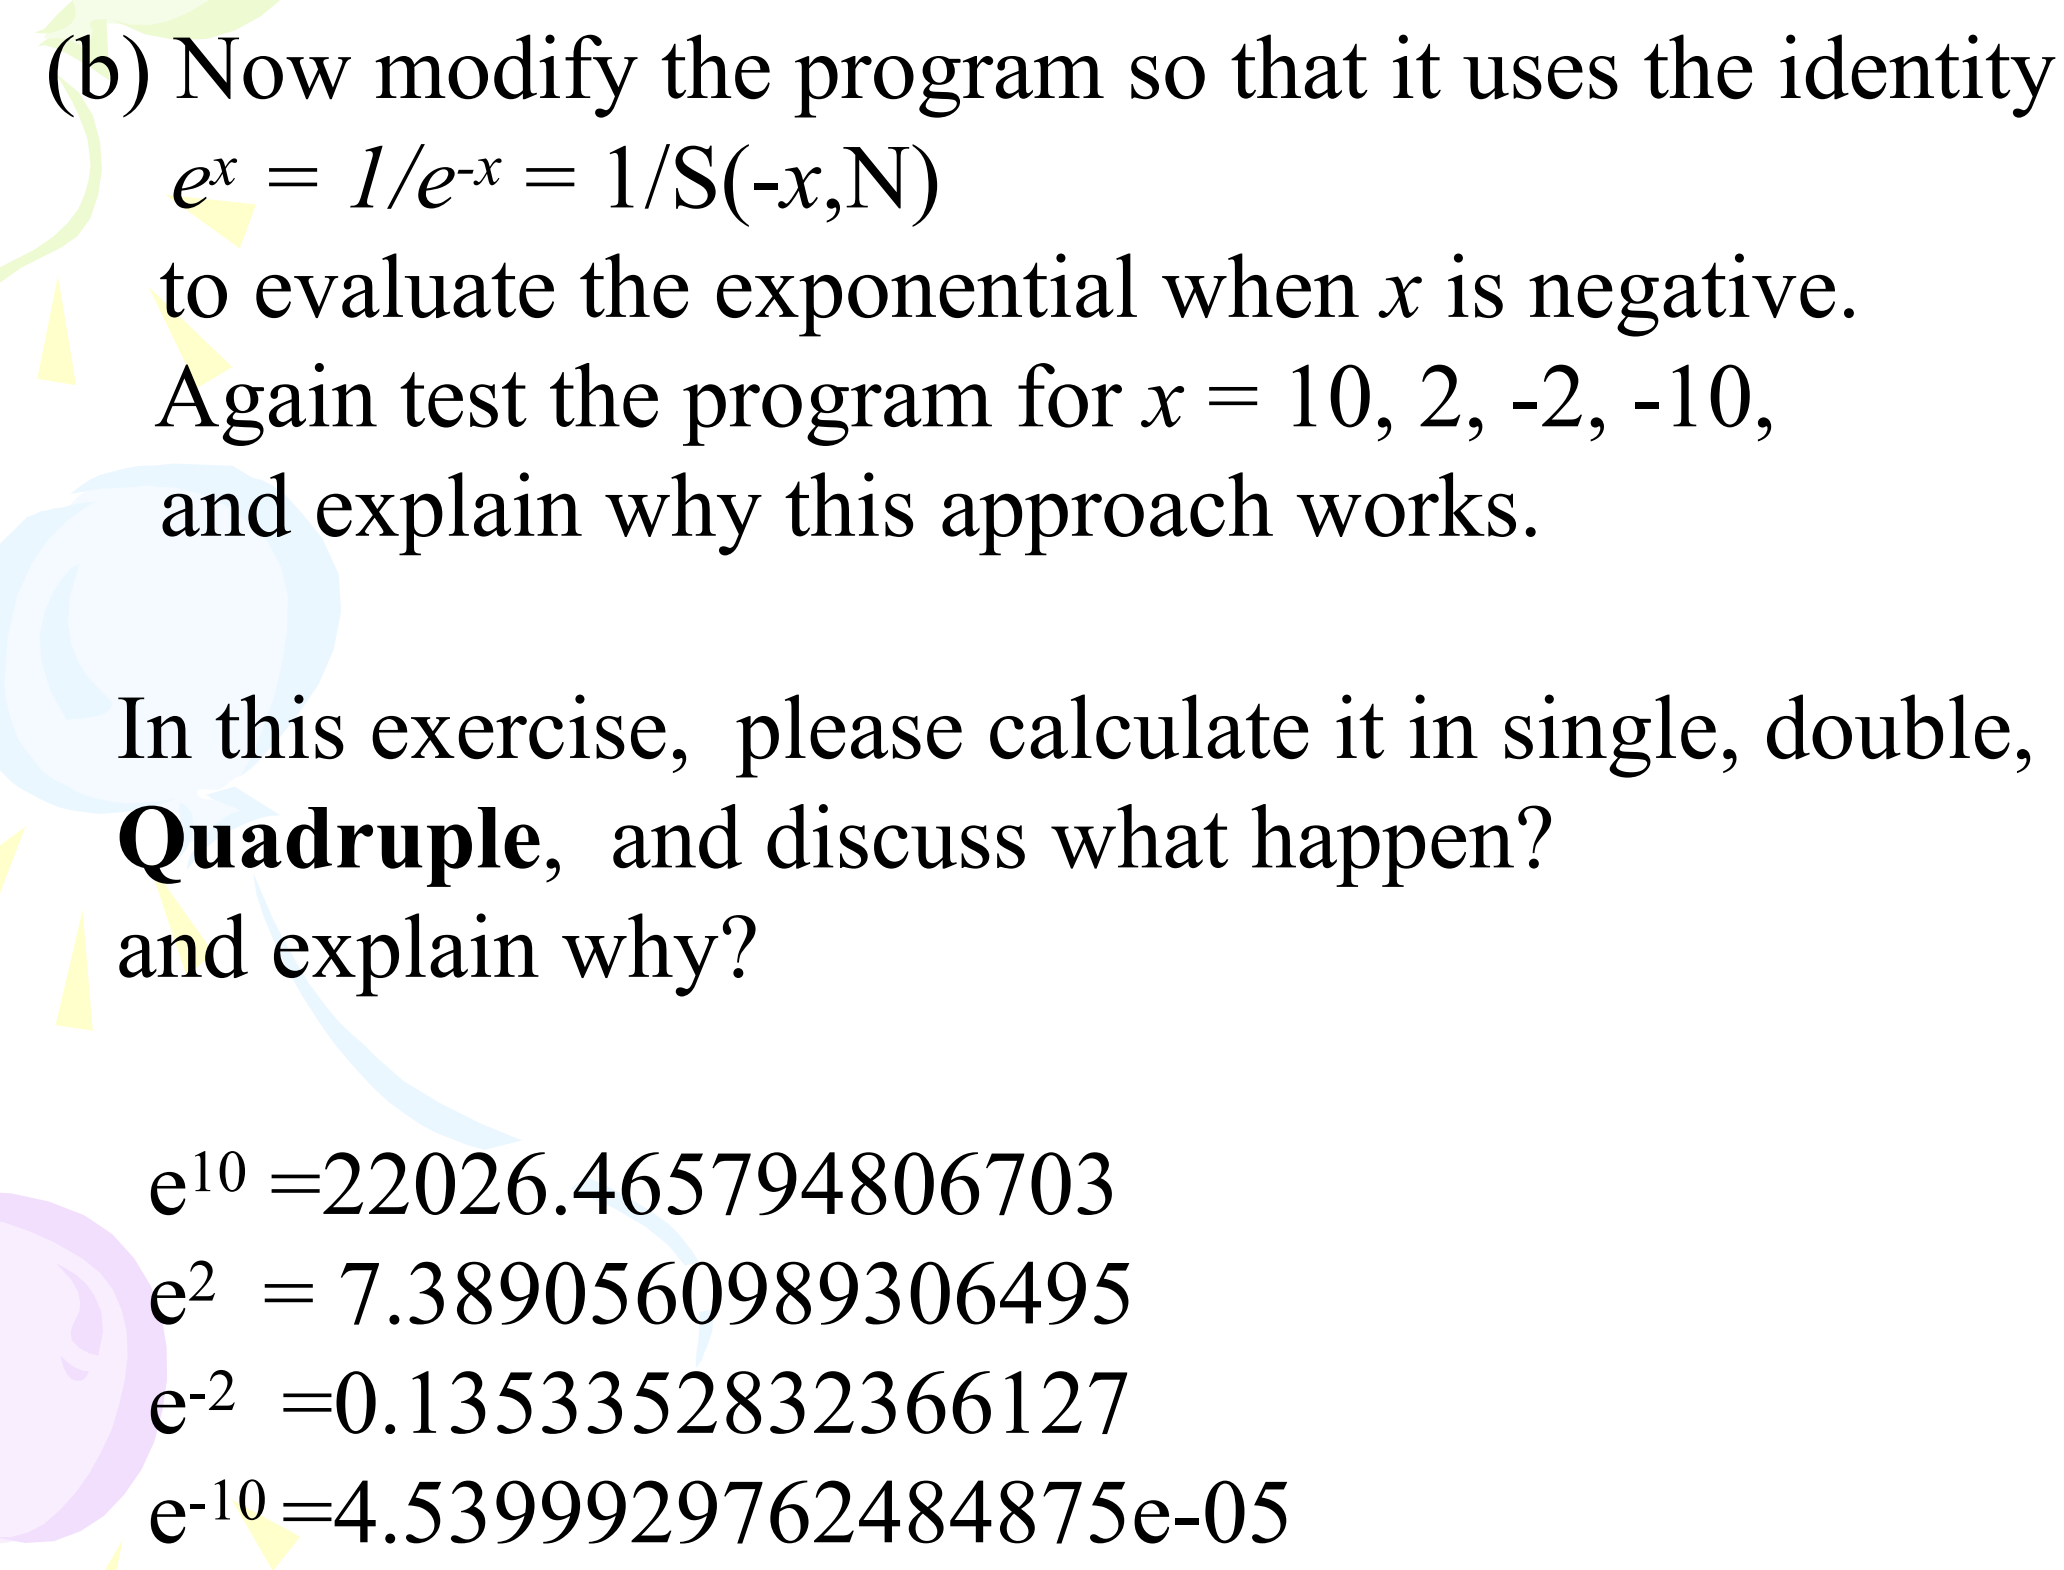
\includegraphics[width=0.7\textwidth]{pic/problem2.png}
\end{figure}

\newpage
\tableofcontents
\newpage

% =================================================
% Part 1
% =================================================
\section{Source Code}

\begin{lstlisting}[language=C++]
#include <iostream>
#include <iomanip>
#include <cmath>
#include <string>
#include <vector>
#include <quadmath.h>

using namespace std;

// ============================================================
// __float128 转字符串
// ============================================================
string qtos(__float128 x, const char* fmt = "%.36Qg") {
    char buf[256];
    quadmath_snprintf(buf, sizeof(buf), fmt, x);
    return string(buf);
}

// ============================================================
// 直接 Taylor 部分和
// S(x,N) = sum_{n=0}^{N} x^n / n!
// ============================================================
template <typename T>
T S_direct(T x, int N) {
    T sum = 1;
    T term = 1;
    for (int n = 1; n <= N; ++n) {
        term = term * x / static_cast<T>(n);
        sum += term;
    }
    return sum;
}

// ============================================================
// 改进方法：x<0 时使用 e^x = 1 / S(-x,N)
// ============================================================
template <typename T>
T S_improved(T x, int N) {
    if (x < 0) {
        return static_cast<T>(1) / S_direct(-x, N);
    } else {
        return S_direct(x, N);
    }
}

// ============================================================
// 精确 exp
// ============================================================
float exact_exp(float x) { return expf(x); }
double exact_exp(double x) { return exp(x); }
__float128 exact_exp(__float128 x) { return expq(x); }

// ============================================================
// 误差
// ============================================================
template <typename T>
T abs_error(T approx, T exact) {
    return fabs(approx - exact);
}

__float128 abs_error(__float128 approx, __float128 exact) {
    return fabsq(approx - exact);
}

template <typename T>
T rel_error(T approx, T exact) {
    if (exact == static_cast<T>(0)) return static_cast<T>(0);
    return fabs((approx - exact) / exact);
}

__float128 rel_error(__float128 approx, __float128 exact) {
    if (exact == 0) return 0;
    return fabsq((approx - exact) / exact);
}

// ============================================================
// 普通打印
// ============================================================
template <typename T>
void print_value(const string& label, T value) {
    cout << left << setw(32) << label
         << setprecision(18) << value << "\n";
}

void print_value_q(const string& label, __float128 value) {
    cout << left << setw(32) << label
         << qtos(value, "%.36Qg") << "\n";
}

// ============================================================
// 每个测试点的结果打印（float）
// ============================================================
void print_case_float(float x, int N) {
    float direct = S_direct<float>(x, N);
    float improved = S_improved<float>(x, N);
    float exact = exact_exp(x);

    cout << "------------------------------------------------------------\n";
    cout << "x = " << x << "\n";
    print_value("Direct Taylor S(x,N) =", direct);
    print_value("Improved value       =", improved);
    print_value("std::exp(x)          =", exact);
    print_value("Abs error of direct  =", abs_error(direct, exact));
    print_value("Rel error of direct  =", rel_error(direct, exact));
    print_value("Abs error improved   =", abs_error(improved, exact));
    print_value("Rel error improved   =", rel_error(improved, exact));
    cout << "\n";
}

// ============================================================
// 每个测试点的结果打印（double）
// ============================================================
void print_case_double(double x, int N) {
    double direct = S_direct<double>(x, N);
    double improved = S_improved<double>(x, N);
    double exact = exact_exp(x);

    cout << "------------------------------------------------------------\n";
    cout << "x = " << x << "\n";
    print_value("Direct Taylor S(x,N) =", direct);
    print_value("Improved value       =", improved);
    print_value("std::exp(x)          =", exact);
    print_value("Abs error of direct  =", abs_error(direct, exact));
    print_value("Rel error of direct  =", rel_error(direct, exact));
    print_value("Abs error improved   =", abs_error(improved, exact));
    print_value("Rel error improved   =", rel_error(improved, exact));
    cout << "\n";
}

// ============================================================
// 每个测试点的结果打印（quadruple）
// ============================================================
void print_case_quad(__float128 x, int N) {
    __float128 direct = S_direct<__float128>(x, N);
    __float128 improved = S_improved<__float128>(x, N);
    __float128 exact = exact_exp(x);

    cout << "------------------------------------------------------------\n";
    cout << "x = " << qtos(x, "%.20Qg") << "\n";
    print_value_q("Direct Taylor S(x,N) =", direct);
    print_value_q("Improved value       =", improved);
    print_value_q("expq(x)              =", exact);
    print_value_q("Abs error of direct  =", abs_error(direct, exact));
    print_value_q("Rel error of direct  =", rel_error(direct, exact));
    print_value_q("Abs error improved   =", abs_error(improved, exact));
    print_value_q("Rel error improved   =", rel_error(improved, exact));
    cout << "\n";
}

// ============================================================
// 每组算完后的分析
// ============================================================
void explain_single_group() {
    cout << "================ SINGLE PRECISION ANALYSIS =================\n";
    cout << "1) In single precision, the number of significant digits is limited.\n";
    cout << "2) For x > 0, the Taylor series terms are all positive, so the summation is relatively stable.\n";
    cout << "3) For x < 0, the series becomes alternating, which means large positive and negative terms\n";
    cout << "   cancel each other.\n";
    cout << "4) This cancellation causes severe round-off loss in float arithmetic.\n";
    cout << "5) Therefore, direct S(x,N) is usually poor for negative x, especially for x = -10.\n";
    cout << "6) The improved formula e^x = 1 / S(-x,N) avoids this cancellation and is much more stable.\n";
    cout << "============================================================\n\n";
}

void explain_double_group() {
    cout << "================ DOUBLE PRECISION ANALYSIS =================\n";
    cout << "1) Double precision keeps more significant digits than single precision.\n";
    cout << "2) Therefore, round-off error is smaller and the results are generally better.\n";
    cout << "3) However, for x < 0, cancellation still exists in the direct Taylor sum.\n";
    cout << "4) So even though double is better than float, direct summation may still lose accuracy\n";
    cout << "   when x is sufficiently negative.\n";
    cout << "5) The improved reciprocal method remains more reliable for negative x.\n";
    cout << "============================================================\n\n";
}

void explain_quad_group() {
    cout << "============== QUADRUPLE PRECISION ANALYSIS ================\n";
    cout << "1) Quadruple precision preserves far more digits than float or double.\n";
    cout << "2) Because of that, the direct Taylor result is improved significantly.\n";
    cout << "3) Even for negative x, cancellation becomes less destructive than before.\n";
    cout << "4) However, the direct formula is still not the best numerical algorithm for x < 0.\n";
    cout << "5) The identity e^x = 1 / S(-x,N) is still the more stable and preferred approach.\n";
    cout << "6) This shows that increasing precision helps, but using a stable algorithm helps even more.\n";
    cout << "============================================================\n\n";
}

// ============================================================
// 整体总分析
// ============================================================
void final_explanation() {
    cout << "==================== FINAL DISCUSSION ======================\n";
    cout << "Part (a): Why does direct S(x,N) fail for x < 0?\n";
    cout << "Because when x is negative, the Taylor series becomes alternating:\n";
    cout << "1 - |x| + |x|^2/2! - |x|^3/3! + ...\n";
    cout << "The intermediate terms can be large, but the final answer e^x is small.\n";
    cout << "So the final result is obtained by subtracting nearly equal large numbers.\n";
    cout << "This is called catastrophic cancellation, and it destroys significant digits.\n\n";

    cout << "Part (b): Why does the improved method work?\n";
    cout << "For x < 0, write e^x = 1 / e^{-x}.\n";
    cout << "Now -x is positive, so S(-x,N) is a sum of positive terms.\n";
    cout << "That summation is numerically stable, and then taking the reciprocal gives a much better result.\n\n";

    cout << "What happens in single, double, and quadruple precision?\n";
    cout << "1) Single precision is affected the most by cancellation.\n";
    cout << "2) Double precision reduces round-off and improves accuracy.\n";
    cout << "3) Quadruple precision improves further and can preserve many more digits.\n";
    cout << "4) But the main lesson is that a numerically stable method is more important than only using higher precision.\n\n";

    cout << "Overall conclusion:\n";
    cout << "For x > 0, direct Taylor summation is fine.\n";
    cout << "For x < 0, the stable choice is e^x = 1 / S(-x,N).\n";
    cout << "============================================================\n";
}

// ============================================================
// 主程序
// ============================================================
int main() {
    cout << fixed;
    int N = 20;

    // ======================== SINGLE =========================
    cout << "######################## FLOAT TESTS ########################\n\n";
    vector<float> xs_float = {10.0f, 2.0f, -2.0f, -10.0f};
    for (float x : xs_float) {
        print_case_float(x, N);
    }
    explain_single_group();

    // ======================== DOUBLE =========================
    cout << "####################### DOUBLE TESTS ########################\n\n";
    vector<double> xs_double = {10.0, 2.0, -2.0, -10.0};
    for (double x : xs_double) {
        print_case_double(x, N);
    }
    explain_double_group();

    // ====================== QUADRUPLE ========================
    cout << "##################### QUADRUPLE TESTS #######################\n\n";
    vector<__float128> xs_quad = {10.0Q, 2.0Q, -2.0Q, -10.0Q};
    for (__float128 x : xs_quad) {
        print_case_quad(x, N);
    }
    explain_quad_group();

    // ======================== FINAL ==========================
    final_explanation();

    return 0;
}
\end{lstlisting}

% =================================================
% Part 3
% =================================================
\section{Numerical Method}

\subsection*{Direct Taylor Approximation}

The direct approximation is defined by
\[
S(x,N)=1+x+\frac{x^2}{2!}+\frac{x^3}{3!}+\cdots+\frac{x^N}{N!}.
\]

In the program, this sum is evaluated iteratively. Instead of computing powers and factorials separately, the \(n\)-th term is generated from the previous one through the recurrence
\[
\text{term}_n=\text{term}_{n-1}\cdot \frac{x}{n}.
\]

This avoids repeated computation and is more efficient than evaluating powers and factorials independently.

\subsection*{Improved Formula for Negative \(x\)}

When \(x<0\), the program uses the identity
\[
e^x=\frac{1}{e^{-x}}\approx \frac{1}{S(-x,N)}.
\]

Thus, for negative \(x\), the approximation is obtained by first evaluating \(S(-x,N)\) and then taking the reciprocal.

\subsection*{Error Measurement}

For each tested value, the program compares the approximation with the standard exponential function. It also computes the absolute error
\[
\text{absolute error}=|\text{approx}-\text{exact}|,
\]
and the relative error
\[
\text{relative error}=\left|\frac{\text{approx}-\text{exact}}{\text{exact}}\right|.
\]

These quantities allow us to evaluate the approximation in both absolute scale and relative scale.

% =================================================
% Part 4
% =================================================
\section{Program Output}

Below is the output of the program in text form.

\subsection*{Single Precision Results}

\begin{lstlisting}
######################## FLOAT TESTS ########################

------------------------------------------------------------
x = 10
Direct Taylor S(x,N) = 21991.484375
Improved value       = 21991.484375
std::exp(x)          = 22026.46484375
Abs error of direct  = 34.98046875
Rel error of direct  = 0.001588110928423703
Abs error improved   = 34.98046875
Rel error improved   = 0.001588110928423703

------------------------------------------------------------
x = 2
Direct Taylor S(x,N) = 7.389056682586669922
Improved value       = 7.389056682586669922
std::exp(x)          = 7.389056205749511719
Abs error of direct  = 4.76837158203e-07
Rel error of direct  = 6.4532891031e-08
Abs error improved   = 4.76837158203e-07
Rel error improved   = 6.4532891031e-08

------------------------------------------------------------
x = -2
Direct Taylor S(x,N) = 0.135335251688957214
Improved value       = 0.135335266590118408
std::exp(x)          = 0.135335281491279602
Abs error of direct  = 2.9802322388e-08
Rel error of direct  = 2.2011035185e-07
Abs error improved   = 1.4901161194e-08
Rel error improved   = 1.10105517592e-07

------------------------------------------------------------
x = -10
Direct Taylor S(x,N) = 13.396759033203125
Improved value       = 0.000045472144847736
std::exp(x)          = 0.000045399930968415
Abs error of direct  = 13.3967132568359375
Rel error of direct  = 295082.25
Abs error improved   = 7.22138779321e-08
Rel error improved   = 0.001590616535395384
\end{lstlisting}

\subsection*{Double Precision Results}

\begin{lstlisting}
####################### DOUBLE TESTS ########################

------------------------------------------------------------
x = 10
Direct Taylor S(x,N) = 21991.482025665063702
Improved value       = 21991.482025665063702
std::exp(x)          = 22026.465794806717895
Abs error of direct  = 34.983769141654193
Rel error of direct  = 0.001588260661858085
Abs error improved   = 34.983769141654193
Rel error improved   = 0.001588260661858085

------------------------------------------------------------
x = 2
Direct Taylor S(x,N) = 7.389056098930604222
Improved value       = 7.389056098930604222
std::exp(x)          = 7.389056098930650407
Abs error of direct  = 4.6185e-14
Rel error of direct  = 6.25e-15
Abs error improved   = 4.6185e-14
Rel error improved   = 6.25e-15

------------------------------------------------------------
x = -2
Direct Taylor S(x,N) = 0.135335283236650394
Improved value       = 0.135335283236613535
std::exp(x)          = 0.135335283236612702
Abs error of direct  = 3.7692e-14
Rel error of direct  = 2.78509e-13
Abs error improved   = 8.33e-16
Rel error improved   = 6.153e-15

------------------------------------------------------------
x = -10
Direct Taylor S(x,N) = 13.396865995695904417
Improved value       = 0.000045472151391750
std::exp(x)          = 0.000045399929762485
Abs error of direct  = 13.396820595766141
Rel error of direct  = 295084.610611805
Abs error improved   = 7.2221629266e-08
Rel error improved   = 0.001590787246663228
\end{lstlisting}

\subsection*{Quadruple Precision Results}

\begin{lstlisting}
##################### QUADRUPLE TESTS #######################

------------------------------------------------------------
x = 10
Direct Taylor S(x,N) = 21991.482025665063142562264368231715
Improved value       = 21991.482025665063142562264368231715
expq(x)              = 22026.465794806716516957900645284245
Abs error of direct  = 34.983769141653374395636277052530065
Rel error of direct  = 0.001588260661858048160301285892311690

------------------------------------------------------------
x = 2
Direct Taylor S(x,N) = 7.389056098930650943441442201050009
Improved value       = 7.389056098930650943441442201050009
expq(x)              = 7.389056098930650227230427460575008
Abs error of direct  = 4.513288628324047e-14
Rel error of direct  = 6.108071948428181e-15

------------------------------------------------------------
x = -2
Direct Taylor S(x,N) = 0.135335283236650307195224317368821724
Improved value       = 0.135335283236613518531646665114144396
expq(x)              = 0.135335283236612691893999494972484395
Abs error of direct  = 3.7615301224822396e-14
Rel error of direct  = 2.7794157092838749e-13
Abs error improved   = 8.2663764717014166e-16
Rel error improved   = 6.1080719484282189e-15

------------------------------------------------------------
x = -10
Direct Taylor S(x,N) = 13.3968659956960410345143055641161008
Improved value       = 4.5472151391750422473095764998242221e-05
expq(x)              = 4.5399929762484851535591515560550610e-05
Abs error of direct  = 13.3968205957662787854966276997260054
Rel error of direct  = 295084.610611808072142149372712087378
Abs error improved   = 7.2221629265570892e-08
Rel error improved   = 0.0015907872466633090
\end{lstlisting}

% =================================================
% Part 5
% =================================================
\section{Discussion}

\subsection*{Why does the direct Taylor sum fail for \(x<0\)?}

When \(x<0\), the Taylor series becomes
\[
e^x = 1-|x|+\frac{|x|^2}{2!}-\frac{|x|^3}{3!}+\cdots.
\]

This is an alternating series. Although the final result \(e^x\) is small, the intermediate terms can be much larger in magnitude. Therefore, the final answer is obtained by cancellation between large positive and negative numbers. In finite precision arithmetic, this cancellation destroys significant digits. This phenomenon is called \textbf{catastrophic cancellation}.

This explains why the direct Taylor approximation becomes unreliable for negative \(x\), especially when \(|x|\) is large. The case \(x=-10\) is the clearest example: the true value is about \(4.54\times 10^{-5}\), while the direct Taylor sum produces a value near \(13.4\), which is completely incorrect.

\subsection*{Why does the improved method work?}

For negative \(x\), we use
\[
e^x=\frac{1}{e^{-x}}\approx \frac{1}{S(-x,N)}.
\]

Now \(-x>0\), so \(S(-x,N)\) is a sum of positive terms. Such a sum is numerically stable, because there is no strong cancellation between terms of opposite sign. After obtaining a stable approximation to \(e^{-x}\), taking the reciprocal gives a much better approximation to \(e^x\).

Thus, the improved method works because it transforms an unstable alternating summation into a stable positive summation.

\subsection*{Effect of Precision}

The numerical experiments show three important facts.

First, increasing precision reduces round-off error. This is why double precision is better than single precision, and quadruple precision is better than double precision for moderate cases.

Second, precision alone cannot solve the instability of the direct Taylor sum for large negative \(x\). Even quadruple precision still gives a disastrous direct result for \(x=-10\).

Third, the improved formula is robust across all three precisions. This means that the dominant factor is not only how many digits are stored, but whether the algorithm is numerically stable.

\vfill
\begin{center}
    \textit{End of Report}
\end{center}

\end{document}